\chapter{Introducción}
\label{chap:introduccion}
Actualmente mucha de nuestra calidad de vida es posible gracias a los bosques, estos además son el hogar de más de la mitad de todas las criaturas y organismos de nuestro planeta. Los bosques dan a la humanidad una variedad de regalos que contribuyen en gran medida a nuestra calidad de vida actual \cite{balvanera2012servicios}.


La deforestación es la pérdida de bosques naturales, algunas de las causas que generan este proceso son: La construcción de carreteras, las actividades agrarias, el desarrollo urbano, la minería ilegal \cite{fearnside2005deforestation}, se puede mencionar algunas consecuencias de la deforestación como son: La pérdida de la biodiversidad, la desertización, inundaciones, desaparición de las selvas tropicales, cambio climático, etc. \cite{garcia2016deforestation}.


Según el MINAGRI (Servicio Nacional Forestal y de Fauna Silvestre) y el MINAM (Programa Nacional de Conservación de Bosques para la Mitigación del Cambio Climático) el Perú registró una deforestación de 164 662 hectáreas de bosques amazónicos en el 2016, cifra que representa un incremento del 5.2\% comparado con el año anterior (156 462 hectáreas). La deforestación en el 2016 es la segunda más alta de los últimos 16 años, solo superada por la registrada en el 2014 (177 566 hectáreas) \cite{noticia1}.


Existen distintos sistemas de monitoreo de cambios de bosques con el fin de detectar deforestación a lo largo del mundo \cite{MinisteriodelambientedelPeru}, actualmente MINAM cuenta con un software de rastreo de deforestación a base de imágenes satelitales, pero este utiliza procesos manuales \cite{MinisteriodelAmbiente}.
%%------------------------------------------------------------------------- %%



\section{Delimitaciones y Definición del Problema}

\subsection{Delimitaciones}
\begin{enumerate}
    \item Aunque existen gran variedad de tipos de cambios solo se tomaran en cuenta aquellos cambios relacionados a los bosques de la Selva Amazónica Peruana.
    \item El tamaño de las imágenes del análisis será de 256 x 256 con una resolución espacial de 3 metros de la plataforma de Planet.
    \item Se tomará las imágenes satelitales ya ortorectificadas para su estudio.
    \item No se validará la georeferenciación de las imágenes de entrada.
    
\end{enumerate}


\subsection{Definición del Problema}

Los cambios de suelos son una medida importante para medir el progreso de la deforestación proporcionando información para tomar medidas en contra de la deforestación. La detección de cambios automatizada basada en imágenes satelitales es una herramienta usada en el análisis de la deforestación, uno de los motivo por el cual un análisis hecho por humanos es costoso es la cantidad de esfuerzo y tiempo que este requiere \cite{SINGH1989}, además que este análisis es propenso a errores, por ejemplo, como se muestra en la \figureautorefname ~\ref{maap} MAAP (Monitoring of the Andean Amazon Project) posee una metodología que consta de los siguientes pasos: 
\begin{enumerate}
    \item Alertas provistas por software de terceros.
    \item Verificación usando imágenes LandSat.
    \item Se obtienen imágenes de alta resolución  para realizar los análisis correspondientes.
    \item En caso de encontrar se utilizan imágenes radar.
    \item Análisis los resultados obtenidos mediante un proceso manual.
    \item Revisar los resultados obtenidos.
    \item Publicar en la plataforma de \gls{MAAP}.
\end{enumerate}{}
.

\begin{figure}[H]

\centering
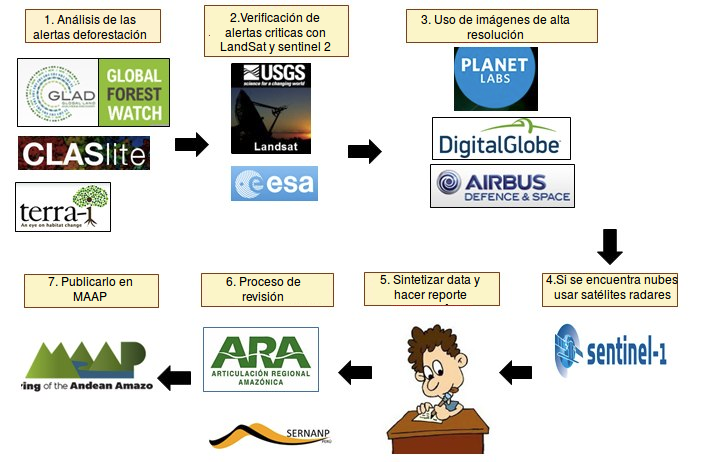
\includegraphics[width=0.8\textwidth]{MetologiaMAAPv2.png}
\caption{Metodología de \gls{MAAP} obtenida de \cite{AmazonConservation} }
\label{maap}

\end{figure}

Algunos de los sistemas de detección de cambios usados para el análisis forestal en el Perú están basados en imágenes de mediana resolución adquiridas mediante convenio con instituciones extranjeras, al hacer un análisis más detallado de las zonas deforestadas se evidencia que las imágenes de mediana resolución(15 metros) no son suficientes \cite{hansen2013high}.

La detección de cambios en imágenes multitemporales es un problema clásico de la teledetección \cite{Zhu2017}, se han desarrollado varios trabajos que tratan de analizar los cambios con técnicas de procesamiento de imágenes tradicionales\cite{AlenCastro2015,Anwar2012,Hirschmugl2014,Zhu2014,hansen2013high}, sin embargo el uso del aprendizaje profundo aun tiene bastante campo de estudio.

\section{Descripción del problema y estudio de las variables}
\label{sec:ideacentral}


\subsection{Variable dependiente e independiente}
Llamamos independiente a la variable cuya asociación o influencia en la variable dependiente es lo que se pretende descubrir en la investigación, es controlada por nosotros los investigadores, en este trabajo de acuerdo a su definición la variable independiente es la imagen satelital y la variable dependiente es el modelo.\\
\subsection{Indicadores de validez}
Para poder evaluar si la detección del cambio esta funcionando apropiadamente es necesario establecer métricas que evalúen que tan precisos hemos sido evaluando el cambio, una medida utilizada es la selección de puntos aleatorios estratificados dicha técnica fue utilizada en papers como \cite{Lunetta2006 ,Olofsson2016 ,Diniz2015}, esta técnica combinada con la información de focos de deforestación provista por \gls{MAAP}\footnote{https://maaproject.org/2019/hotspot-peru-2018/}  serán utilizadas para validar la correcta detección de cambios. La técnica de puntos estratificados sera  definida en la sección \ref{subsection:validacion}.
%% ------------------------------------------------------------------------- %%
\section{Objetivos}
\label{sec:objetivo}

\subsection{Objetivo general}
Realizar un modelo computacional para la detección de cambios de la selva amazónica usando imágenes satélites multiespectrales mediante un enfoque de aprendizaje profundo.
\subsection{Objetivos específicos}
Para lograr un modelo computacional correcto  debemos de resolver los siguientes problemas:
\begin{enumerate}
  \item Elaborar una base de datos de imágenes satelitales.


 \item Construir un modelo de red neuronal que permita la segmentación semántica de cada imagen.

 \item Elaborar un modelo que permita realizar un mapa de cambios. 
\item Evaluación de resultados.
\end{enumerate}

\section{Hipótesis}
Un modelo computacional basado en deep learning puede superar los resultados hechos mediante las técnicas tradicionales de procesamiento de imágenes para el problema de detección de cambios.


\section{Justificación}
Se puede entender a la deforestación como el proceso por el cual la superficie forestal es destruida, de esta manera la detección de cambios puede ser usada como un método de detección de deforestación.   

%El cambio de suelos da un indicio de como se da el proceso de deforestación, es por eso que la detección de cambios provee información de soporte para la prevención de la deforestación.

%Encontrar zonas deforestadas puede ser difícil si se trata de realizar mediante una exploración desde el suelo, es por eso que en la actualidad se usan distintas herramientas como imágenes satelitales, fotografías áreas, etc. 

Las imágenes satelitales son de gran ayuda para el análisis de suelos, estas imágenes pueden llegar a zonas donde el acceso es difícil \cite{AlenCastro2015}. El uso de imágenes satelitales es una solución más barata en comparación a la toma de fotografías aéreas, además las imágenes satelitales cuentan con más información que la posiblemente obtenible mediante la vista humana \cite{unsalan2013multispectral}.


Hace algunos años la adquisición de imágenes satelitales era un problema, actualmente se cuenta con varios repositorios de imágenes libres como son: Earth Obsevation System\footnote{https://eos.com/}, Planet\footnote{https://www.planet.com/} o United States Geological Survey Digital Spectral Library\footnote{https://speclab.cr.usgs.gov/spectral-lib.html}; también existen algunas fuentes de datos libres como es el del concurso ``Understanding the Amazon from Space'' de Kaggle\footnote{https://www.kaggle.com/c/planet-understanding-the-amazon-from-space}. 


El Perú adquirió un satélite de alta resolución llamado PeruSat que provee amplia información para los distintos estudios que se deseen realizar, para solicitar imágenes de PeruSat solo es necesario establecer un convenio con CONIDA (Comisión Nacional de Investigación y Desarrollo Aeroespacial).

Las técnicas de aprendizaje profundo han sido usadas en distintas tareas, recientemente se ha comenzado a usar estas técnicas en la teledetección \cite{zhang2016deep} debido a las ventajas que ofrece en problemas de alta dificultad, en cuyos casos no es posible una extracción de características apropiada.

 El aprendizaje profundo es un enfoque en el cual las características no son necesariamente tomadas a mano, por eso el enfoque profundo puede ser útil para el problema de la detección de cambios, dado que algunas características pueden no ser halladas a mano.
 \section{Alcances}
El modelo sera viable para imágenes que no presenten demasiado tamaño.










\section{Metodología}
La detección de cambios se hará utilizando técnicas de aprendizaje profundo.

La investigación se dividirá en 3 etapas. 
\begin{enumerate}
\item La primera etapa sera la construcción de una base de datos apropiada incluye:
\begin{itemize}
 \item Recolección de imágenes satelitales de distintas fuentes (Kaggle, Planet, PeruSat).
 \item Procesamiento de las imágenes para correcciones geométricas o atmosféricas.
 \item Segmentación manual de las imágenes con su respectivo etiquetado. 
\end{itemize}
\item En la segunda etapa se construirá un modelo de red convolucional para poder realizar un segmentado semántico a cada uno de los píxeles de las imágenes.

%http://lema.rae.es/dpd/srv/search?key=p%EDxel

\item Para concluir se usaran los resultados para construir un modelo computacional adecuado basado en el articulo de \cite{doshi2018satellite} para obtener una imagen segmentada.
\end{enumerate}
\begin{figure}[H]
    \centering
    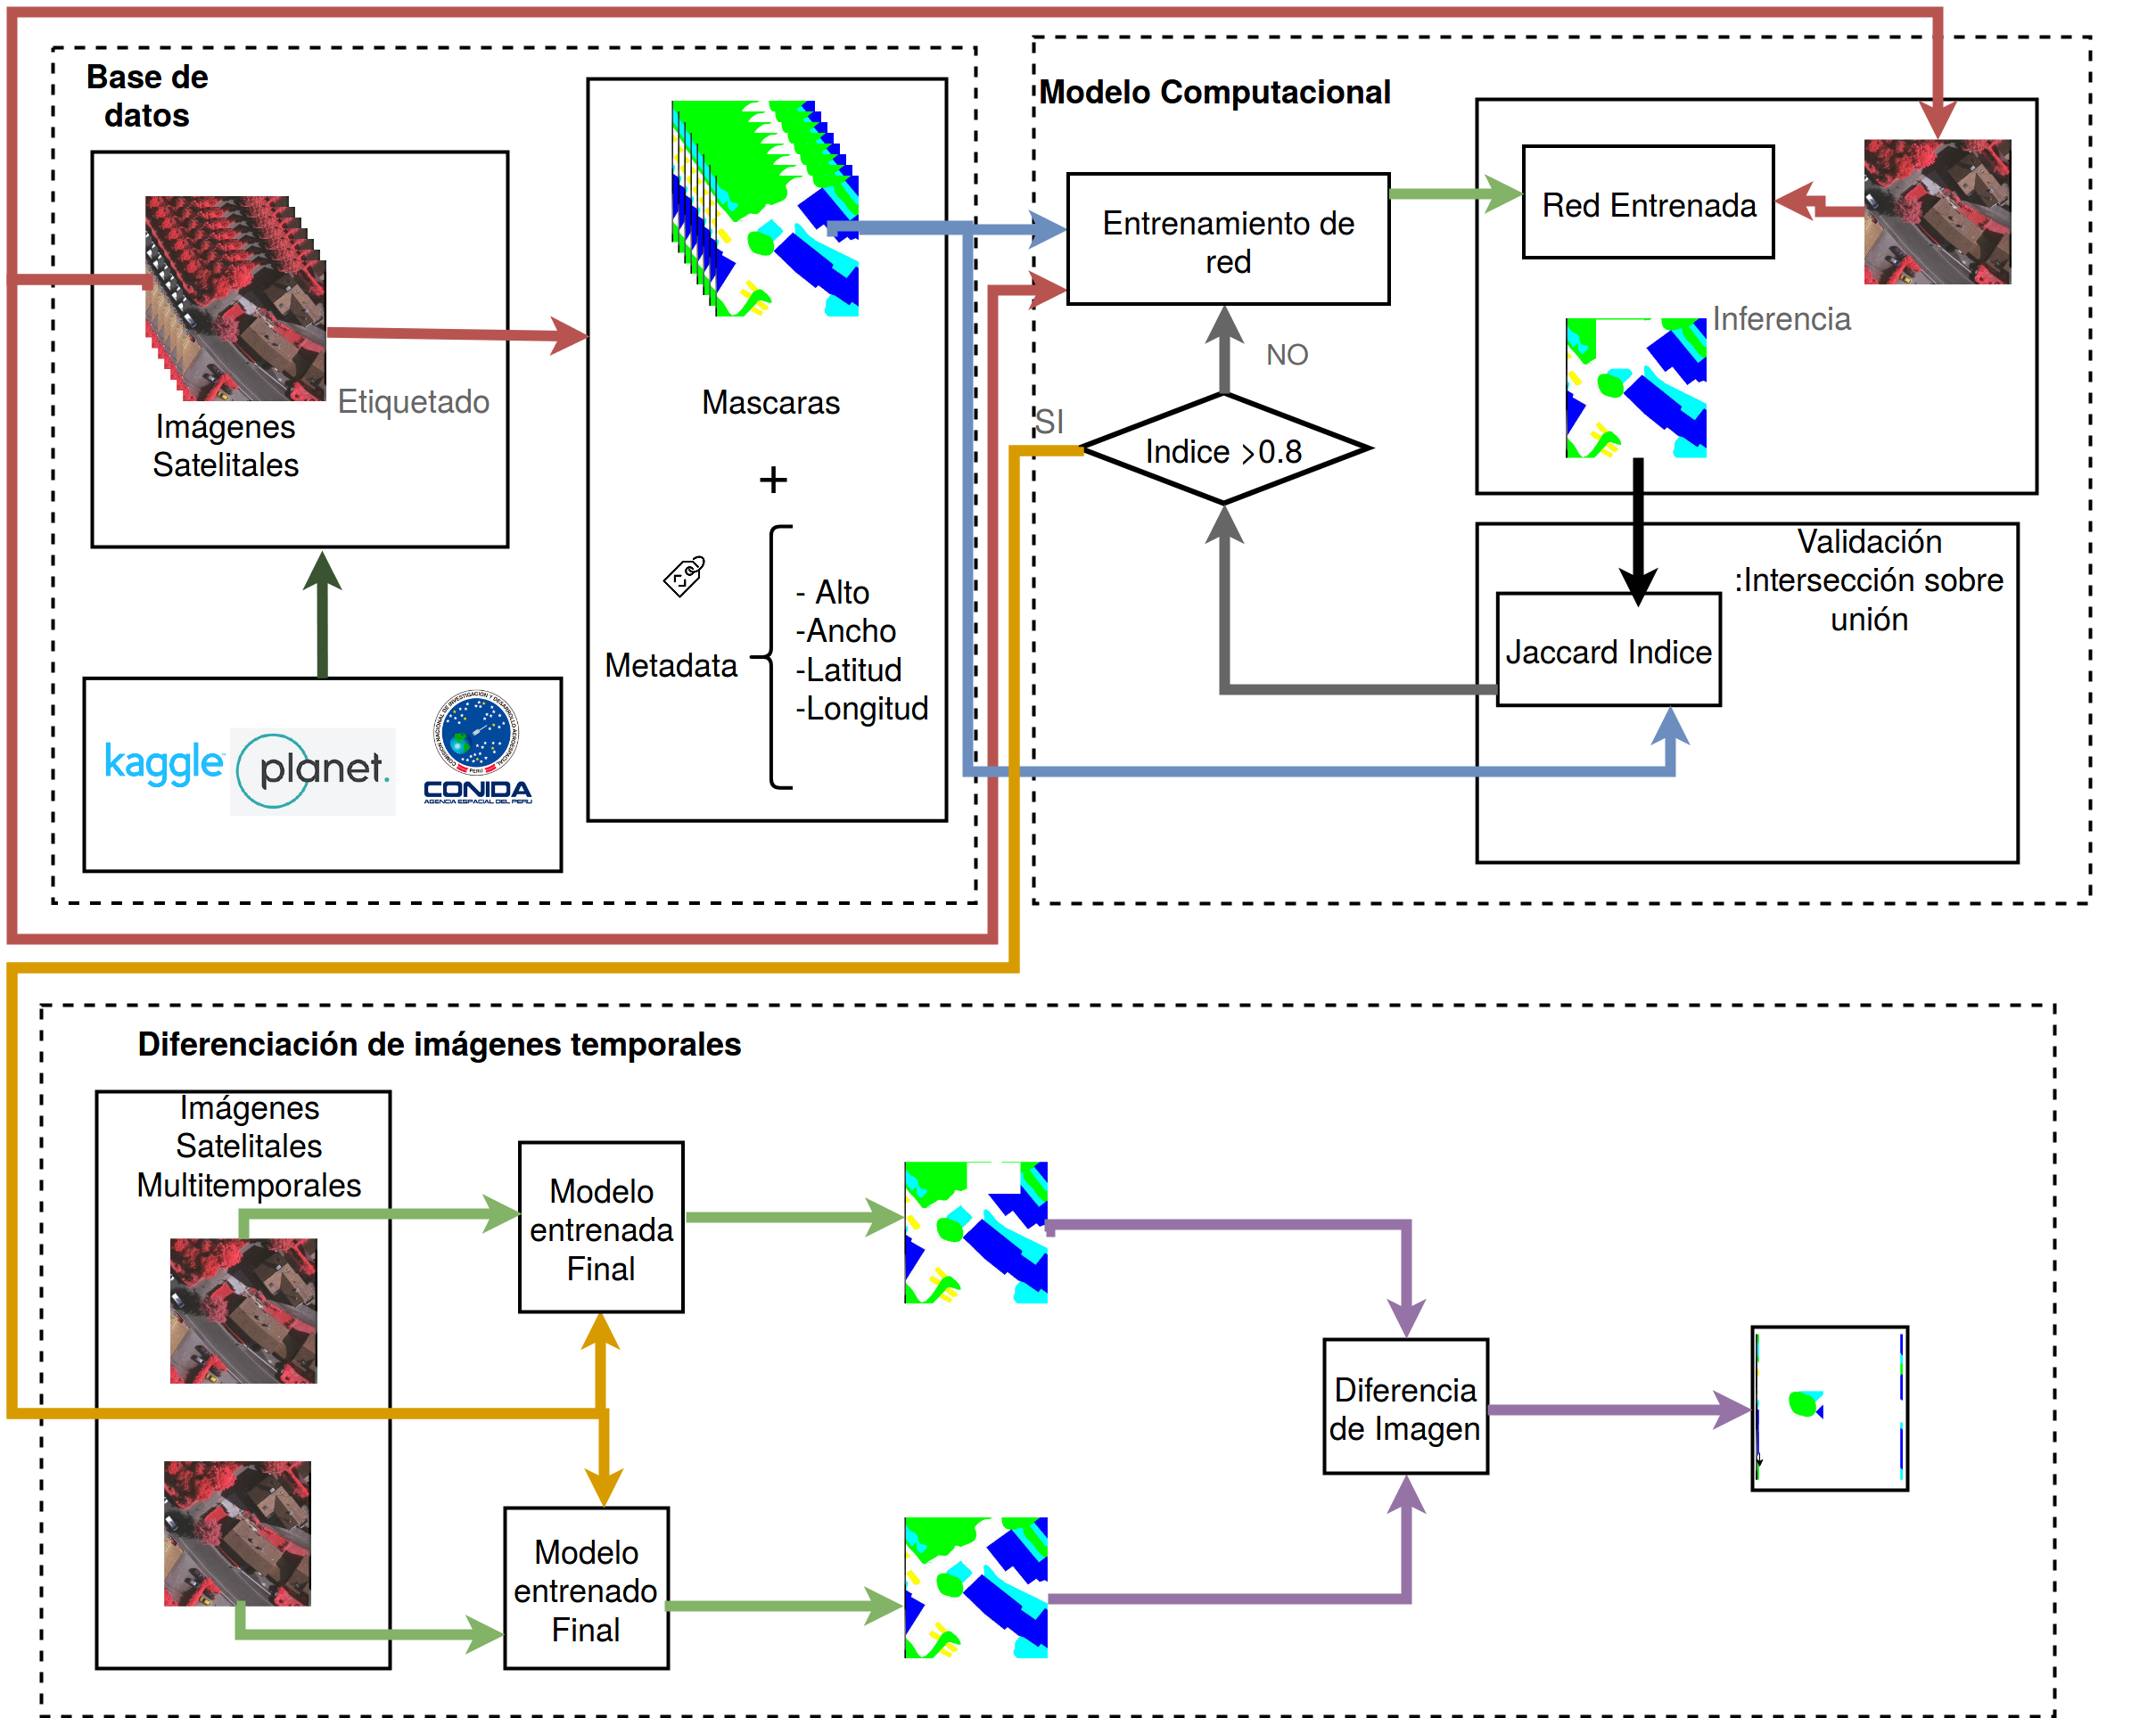
\includegraphics[width=0.8\textwidth]{images/ArquitecturaFinal.png}
    \caption{Gráfico de la metodología}
    \label{fig:my_label}
\end{figure}
%% ------------------------------------------------------------------------- %%
\section{Organización del trabajo}
A continuación y a modo de guía de la lectura del documento, se describe la estructura de la tesis y los contenidos esenciales de cada capítulo.
\begin{itemize}
\item Capítulo \ref{chap:introduccion} (\textit{Introducción}): Se especifica el planteamiento del problema, las variables dependiente e independiente, los objetivos, así como la metodología empleada, y la organización de la tesis.
\item Capítulo \ref{chap:marcoTeorico}(\textit{Marco Teórico:}) Se desarrollaran los conceptos necesarios para poder entender la propuesta.
\item Capítulo \ref{chap:imagenes}(\textit{Base de datos de Imágenes Satelitales}) Se detallara el proceso de construcción de la base de datos.

\item Capítulo \ref{chap:desarrollo}(\textit{Desarrollo}) Se detallara el proceso de construcción del modelo propuesto.


\item Capítulo \ref{chap:pruebas} (\textit{Pruebas y resultados}): Se describen las pruebas realizadas, los diferentes parámetros que se utilizaron para encontrar los resultados, así como la validación de los resultados, la precisión.
\item Capítulo \ref{chap:conclusiones} (\textit{Conclusiones y trabajos futuros}): Finalmente se dan las conclusiones finales de todo el trabajo realizado y se presentan interesantes líneas de trabajo que quedan abiertas a futuras investigaciones.
Anda caliente el cartel el respeto le han faltado 
\end{itemize}

